\documentclass{beamer}
\usetheme{Copenhagen}
\usepackage{graphicx}
\usepackage{svg}
\usepackage{listings}
\title{Introduction to Python}
\subtitle{Lesson 1: Basics}

\begin{document}
\begin{frame}
  \titlepage
\end{frame}

\section{What is Python?}
\begin{frame}[fragile]{Why Python?}
  Python is:
  \begin{itemize}
	\item easy to learn
	\item easy to write (dev time is worth more than runtime)
	\item great for prototyping and scripting but can do powerful stuff too
  \end{itemize}
\end{frame}
\begin{frame}[fragile]{Python 2 vs. Python 3}
  Python has split (for now) between 2 and 3.
  \begin{itemize}
	\item Python 3 is not backwards compatible but differences are small (for us).
	\item Python 2.7 is the last Python 2 version - shutdown is 2020
	\item We are learning Python 2 but the jump is easy!
	\item You are welcome to use Python 3 but look up differences (or ask me)
  \end{itemize}
\end{frame}
\begin{frame}[fragile]{Overview}
  Python is:
  \begin{itemize}
	\item multi-paradigm (object-oriented with functional stuff thrown in),
	\item dynamically typed,
	\item interpreted.
  \end{itemize}
\end{frame}
\begin{frame}[fragile]{Python is Interpreted}
\begin{figure}[!ht]
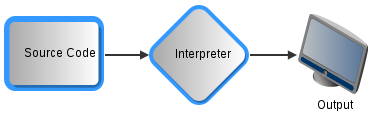
\includegraphics[scale=.7]{380px-Interpreted_Code_Flow_Diagram.png}
\end{figure}
The interpreter is a program called Python.
\end{frame}

\begin{frame}[fragile]{Running Python}
 Two ways of using the Python interpreter (for us):
\begin{itemize}
\item For long programs save your code in a .py file and run
  \begin{block}{}
  \begin{lstlisting}{frame=single}
  python script.py 
  \end{lstlisting}
\end{block}
  .py files are just text files!
  \item For simple calculations just run the interpreter:
  \begin{block}{}
  \begin{lstlisting}{frame=single}
  python 
  \end{lstlisting}
\end{block}
This command will launch the REPL, an interactive mode.
\end{itemize}
\end{frame}

\begin{frame}[fragile]{The REPL}
  The REPL is the default behaviour when you run the interpreter.
  \begin{block}{REPL stands for:}
  	\begin{itemize}
  		\item READ
  		\item EVAL
  		\item PRINT
  		\item LOOP
  	\end{itemize}
  \end{block}
\end{frame}
\begin{frame}
	Example Time!
\end{frame}
\end{document}
